%% Requires compilation with XeLaTeX 
\documentclass[10pt,xcolor={table,dvipsnames},t]{beamer}
\usetheme{UCBerkeley}

\usepackage{graphics,graphicx,float}
\usepackage{multicol}

\title{CP Violation In and Beyond The Standard Model}
\subtitle{Two Higgs Doublet Model Type II Corrections to Flavour Observables}
\author{Matthew Rossetter}
\institute{}
\date{\today}

\graphicspath{{../images/}}

\begin{document}

\section{Introduction}
\begin{frame}
  \titlepage
\end{frame}

% Uncomment these lines for an automatically generated outline.
%\begin{frame}{Outline}
%  \tableofcontents
%\end{frame}
\begin{frame}{The Standard Model}

\end{frame}

\begin{frame}{Unsolved Problems of the Standard Model}

\end{frame}

\begin{frame}{Why Two Higgs Doublet Model?}

\end{frame}


\section{Global Fits}
\begin{frame}{First Inputs}
    \begin{columns}[c]
        \begin{column}{0.33\textwidth}
            \begin{itemize}
                \item $1\sigma$ scan
                \item Leptonic, mixing, and radiative
                \item No real constraint on $\tan\beta$
                \item $m_{H^+} > 340\,$GeV
            \end{itemize}
        \end{column}
        \begin{column}{0.60\textwidth}
            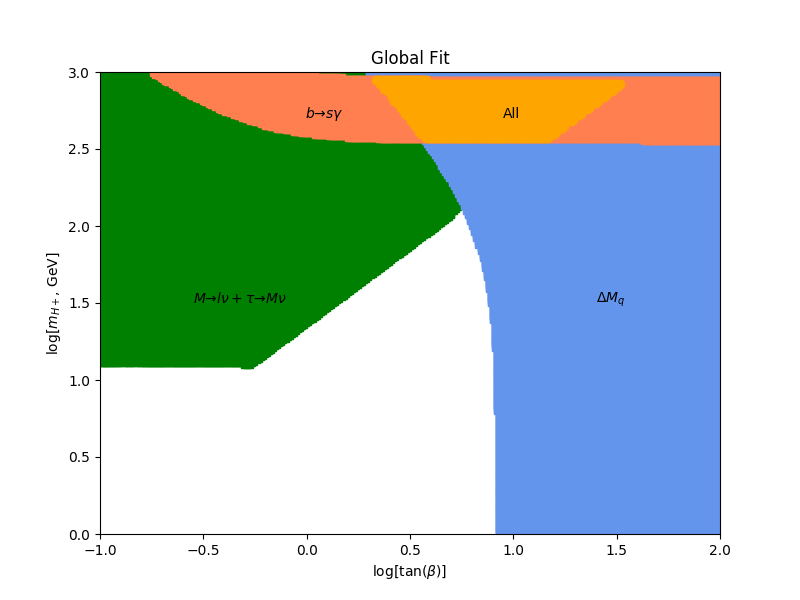
\includegraphics[scale=0.35]{global}
        \end{column}
    \end{columns}
\end{frame}
            %Initial stuff from 0907.5135 here.

\begin{frame}{New Inputs}
    \begin{columns}[c]
        \begin{column}{0.45\textwidth}
            \begin{itemize}
                \item $B_s\to\mu^+\mu^-$ 
                    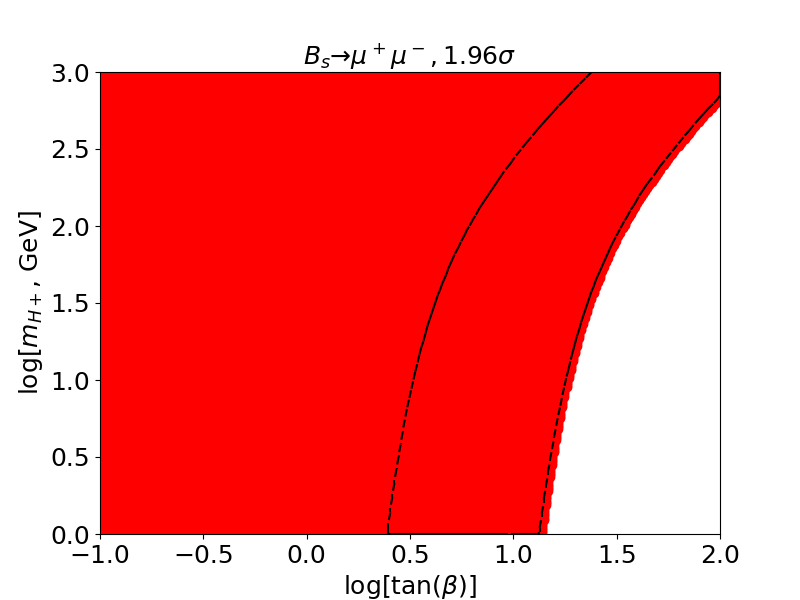
\includegraphics[scale=0.25]{mumu}
            \end{itemize}
        \end{column}
        \begin{column}{0.45\textwidth}
            \begin{itemize}
                \item $R(D^{(*)})$ BOTH 
                    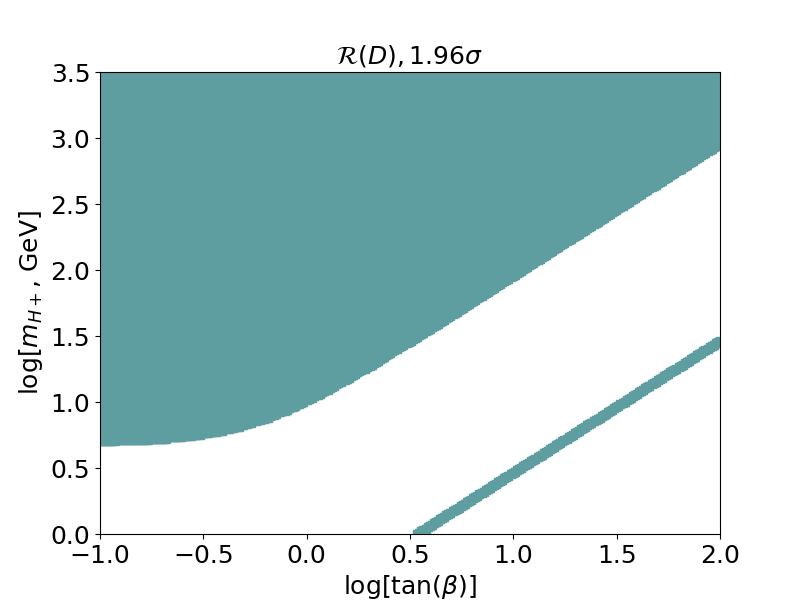
\includegraphics[scale=0.25]{rd_196sig}
            \end{itemize}
        \end{column}
    \end{columns}
\end{frame}

\begin{frame}{Statistical Fitting of Scans}
    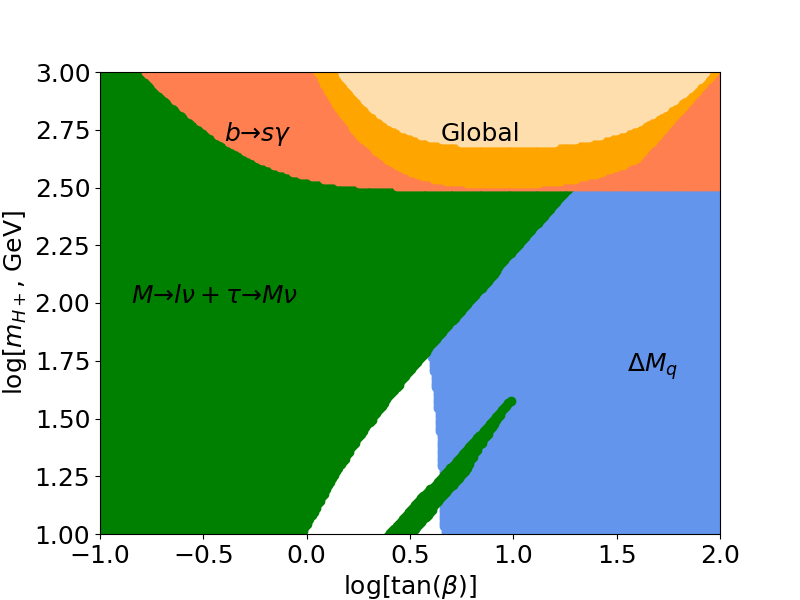
\includegraphics[scale=0.35]{global_08}
\end{frame}

\begin{frame}{Extended Global Fit}
    \begin{columns}[c]
        \begin{column}{0.37\textwidth}
            \begin{itemize}
                \item 95\% CL: $m_{H^+}>390\,$GeV
                \item $1\sigma$: $m_{H^+}>530\,$GeV
                \item $\tan\beta\gtrapprox2$
            \end{itemize}
        \end{column}
        \begin{column}{0.60\textwidth}
            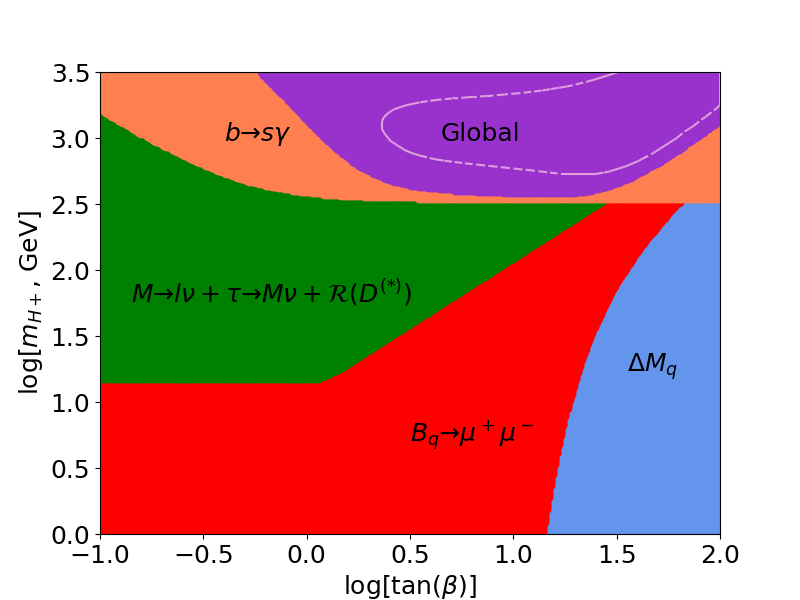
\includegraphics[scale=0.35]{global_lines.png}
        \end{column}
    \end{columns}
\end{frame}

\begin{frame}{CKM Element Modifications}

\end{frame}

\section{Extension to SM4}
\begin{frame}{Four Generations?}

\end{frame}

\begin{frame}{SM4 with 2HDM Type II}

\end{frame}

\section{Questions}
\begin{frame}
    \begin{center}
        \vspace{60pt}
        \Huge Any Questions?
    \end{center}
\end{frame}

\end{document}
